\documentclass{math}

\usepackage{graphicx}

\geometry{letterpaper, margin=0.5in}

\title{Differential Equations: Homework 8}
\author{Alvin Lin}
\date{January 2018 - May 2018}

\begin{document}

\maketitle
\clearpage

\section*{Section 4.10}

\subsubsection*{Exercise 4}
Determine the equation of motion for an undamped system at resonance governed
by:
\[ \ddiff{^2y}{t^2}+y = 5\cos(t) \quad y(0) = 0 \quad y'(0) = 1 \]
Sketch the solution.
\begin{align*}
  y''+y &= 5\cos(t) \\
  r^2+1 &= 0 \\
  r &= 0\pm i \quad \alpha = 0 \quad \beta = 1 \\
  y_h &= c_1\cos(t)+c_2\sin(t) \\
  y_p &= t\bigg[A\cos(t)+B\sin(t)\bigg] = At\cos(t)+Bt\cos(t) \\
  y_p' &= A\cos(t)-At\sin(t)+B\sin(t)+Bt\cos(t) \\
  y_p'' &= -A\sin(t)-\bigg[A\sin(t)+At\cos(t)\bigg]+
    B\cos(t)+\bigg[B\cos(t)-Bt\sin(t)\bigg] \\
  y''+y &= 5\cos(t) \\
  &= -A\sin(t)-A\sin(t)-At\cos(t)+B\cos(t)+B\cos(t)- \\
  &~~~~ Bt\sin(t)+At\cos(t)+Bt\sin(t) \\
  &= -2A\sin(t)+2B\cos(t) \\
  -2A &= 0 \quad 2B = 5 \quad A = 0 \quad B = \frac{5}{2} \\
  y_p &= \frac{5}{2}t\sin(t) \\
  y &= c_1\cos(t)+c_2\sin(t)+\frac{5}{2}t\sin(t) \\
  y' &=
    -c_1\sin(t)+c_2\cos(t)+c_2\cos(t)+\frac{5}{2}\sin(t)+\frac{5}{2}t\cos(t) \\
  y(0) &= 0 = c_1 \\
  y'(0) &= 1 = c_2 \\
  y &= \sin(t)+\frac{5}{2}t\sin(t) \\
  &= (1+\frac{5}{2}t)\sin(t)
\end{align*}
\begin{center}
  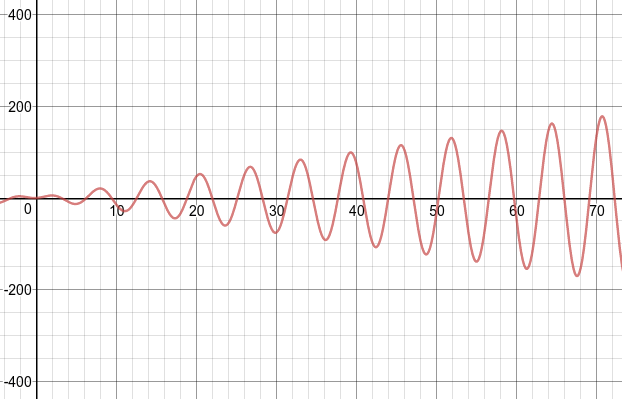
\includegraphics[width=9cm]{assets/hw_09_04.png}
\end{center}

\subsubsection*{Exercise 15}
An 8-kg mass is attached to a string hanging from the ceiling and allowed
to come to rest. Assume that the spring constant is \( 40\frac{N}{m} \) and the
damping constant is \( 3\frac{N\cdot sec}{m} \). At time \( t = 0 \), an
external force of \( 2\sin(2t)\cos(2t) \) N is applied to the system. Determine
the amplitude and frequency of the steady-state solution.
\begin{align*}
  8y''+3y'+40y &= 2\sin(2t)\cos(2t) \\
  8r^2+3r+40 &= 0 \\
  r &= \frac{-3\pm\sqrt{9-4(8)(40)}}{2(8)} \\
  &= -\frac{3}{16}\pm\frac{\sqrt{1271}i}{16} \quad \alpha = -\frac{3}{16} \quad
    \beta = \frac{\sqrt{1271}}{16} \\
  y_h &= \e^{-\frac{3}{16}t}\bigg(c_1\cos(\frac{\sqrt{1271}}{16}t)+
    c_2\sin(\frac{\sqrt{1271}}{16}t)\bigg) \\
  8y''+3y'+40y &= 2\sin(2t)\cos(2t) = \sin(4t) \\
  y_p &= A\cos(4t)+B\sin(4t) \\
  y_p' &= -4A\sin(4t)+4B\cos(4t) \\
  y_p'' &= -16A\cos(4t)-16B\sin(4t)
\end{align*}
\begin{align*}
  8(-16A\cos(4t)-16B\sin(4t))+3(-4A\sin(4t)+4B\cos(4t))+40(A\cos(4t)+B\sin(4t))
    &= \sin(4t) \\
  (-88A+12B)\cos(4t)+(-12A-88B)\sin(4t) &= \sin(4t) \\
  -12A-88B = 1 \quad -88A+12B &= 0 \\
  A = \frac{3}{1972} \quad B &= \frac{11}{986}
\end{align*}
\begin{align*}
  y_p &= \frac{3}{1972}\cos(4t)+\frac{11}{986}\sin(4t) \\
  amplitude &= \sqrt{(\frac{3}{1972})^2+(\frac{11}{986})^2} \\
  \phi &= \arctan(\frac{B}{A}) \approx 82.23 \\
  T &= \frac{2\pi}{\omega} = \frac{2\pi}{4} = \frac{\pi}{2} \\
  f &= \frac{\omega}{2\pi} = \frac{2}{\pi}
\end{align*}

\section*{Section 7.2}

\subsubsection*{Exercise 3}
Use Definition 1 to determine the Laplace transform of the given function.
\begin{align*}
  \laplace{\e^{6t}} &= \int_{0}^{\infty}\e^{-st}\e^{6t}\diff{t} \\
  &= \lim_{N\to\infty}\int_{0}^{N}\e^{6t-st}\diff{t} \\
  &= \lim_{N\to\infty}\int_{0}^{N}\e^{(6-s)t}\diff{t} \\
  &= \lim_{N\to\infty}\bigg[\frac{1}{6-s}\e^{(6-s)t}\bigg]_{0}^{N} \\
  &= 0-\frac{1}{6-s}, \quad s > 6 \\
\end{align*}

\subsubsection*{Exercise 11}
Use Definition 1 to determine the Laplace transform of the given function.
\begin{align*}
  f(t) &= \begin{cases}
    \sin(t), \quad 0<t<1 \\
    0, \quad \pi<t
  \end{cases} \\
  \laplace{f(t)} &= \int_{0}^{\infty}\e^{-st}f(t)\diff{t} \\
  &= \int_{0}^{\pi}\e^{-st}\sin(t)\diff{t}+
    \int_{\pi}^{\infty}\e^{-st}0\diff{t} \\
  &= \int_{0}^{\pi}\e^{-st}\sin(t)\diff{t} \\
  &= \bigg[-\frac{\e^{-st}(s\sin(t)+\cos(t))}{s^2+1}\bigg]_{0}^{\pi} \\
  &= \frac{-\e^{-s\pi}(-1)}{s^2+1}-\frac{-\e^{0}(1)}{s^2+1} \\
  &= \frac{\e^{-s\pi}+1}{s^2+1}
\end{align*}

\subsubsection*{Exercise 13}
Use the Laplace transform table and the linearity of the Laplace transform to
determine the following transforms.
\begin{align*}
  \laplace{6\e^{-3t}-t^2+2t-8} &= 6\laplace{\e^{-3t}}-\laplace{t^2}+
    2\laplace{t}-8\laplace{1} \\
  &= 6(\frac{1}{s+3})-\frac{2!}{s^3}+2(\frac{1}{s^2})-8(\frac{1}{s}) \\
  &= \frac{6}{s+3}-\frac{2}{s^3}+\frac{2}{s^2}-\frac{8}{s}, \quad s>0
\end{align*}

\subsubsection*{Exercise 14}
Use the Laplace transform table and the linearity of the Laplace transform to
determine the following transforms.
\begin{align*}
  \laplace{5-\e^{2t}+6t^2} &= 5\laplace{1}-\laplace{\e^{2t}}+6\laplace{t^2} \\
  &= 5(\frac{1}{s})-\frac{1}{s-2}+6(\frac{2!}{s^3}) \\
  &= \frac{5}{s}-\frac{1}{s-2}+\frac{12}{s^3}, \quad s>2
\end{align*}

\subsubsection*{Exercise 15}
Use the Laplace transform table and the linearity of the Laplace transform to
determine the following transforms.
\begin{align*}
  \laplace{t^3-t\e^t+\e^{4t}\cos(t)} &= \laplace{t^3}-\laplace{t\e^t}+
    \laplace{\e^{4t}\cos(t)} \\
  &= \frac{3!}{s^4}-\frac{1}{(s-1)^2}+\frac{s-4}{(s-4)^2+1^2} \\
  &= \frac{6}{s^4}-\frac{1}{(s-2)^2}+\frac{s-4}{(s-4)^2+1}, \quad s>4
\end{align*}

\subsubsection*{Exercise 16}
Use the Laplace transform table and the linearity of the Laplace transform to
determine the following transforms.
\begin{align*}
  \laplace{t^2-3t-2\e^{-t}\sin(3t)} &=
    \laplace{t^2}-3\laplace{t}-2\laplace{\e^{-t}\sin(3t)} \\
  &= \frac{2}{s^3}-3(\frac{1}{s^2})-2(\frac{3}{(s+1)^2+3^2}) \\
  &= \frac{2}{s^3}-\frac{3}{s^2}-\frac{6}{(s+1)^2+9}, \quad s>0
\end{align*}

\subsubsection*{Exercise 17}
Use the Laplace transform table and the linearity of the Laplace transform to
determine the following transforms.
\begin{align*}
  \laplace{\e^{3t}\sin(6t)-t^3+\e^t} &= \laplace{\e^{3t}\sin(6t)}-
    \laplace{t^3}+\laplace{\e^t} \\
  &= \frac{6}{(s-3)^2+6^2}-\frac{3!}{s^4}+\frac{1}{s-1} \\
  &= \frac{6}{(s-3)^2+36}-\frac{6}{s^4}+\frac{1}{s-1}, \quad s>3
\end{align*}

\subsubsection*{Exercise 18}
Use the Laplace transform table and the linearity of the Laplace transform to
determine the following transforms.
\begin{align*}
  \laplace{t^4-t^2-t+\sin(\sqrt{2}t)} &= \laplace{t^4}-\laplace{t^2}-
    \laplace{t}+\laplace{\sin(\sqrt{2}t)} \\
  &= \frac{4!}{s^5}-\frac{2!}{s^3}-\frac{1!}{s^2}+
    \frac{\sqrt{2}}{s^2+(\sqrt{2})^2} \\
  &= \frac{24}{s^5}-\frac{2}{s^3}-\frac{1}{s^2}+\frac{\sqrt{2}}{s^2+2},
    \quad s>0
\end{align*}

\subsubsection*{Exercise 19}
Use the Laplace transform table and the linearity of the Laplace transform to
determine the following transforms.
\begin{align*}
  \laplace{t^4\e^{5t}-\e^t\cos(\sqrt{7}t)} &= \laplace{t^4\e^{5t}}-
    \laplace{\e^t\cos(\sqrt{7}t)} \\
  &= \frac{4!}{(s-5)^5}-\frac{s-1}{(s-1)^2+(\sqrt{7})^2} \\
  &= \frac{24}{(s-5)^5}-\frac{s-1}{(s-1)^2+7}, \quad s<5
\end{align*}

\subsubsection*{Exercise 20}
Use the Laplace transform table and the linearity of the Laplace transform to
determine the following transforms.
\begin{align*}
  \laplace{\e^{-2t}\cos(\sqrt{3}t)-t^2\e^{-2t}} &=
    \laplace{\e^{-2t}\cos(\sqrt{3}t)}-\laplace{t^2\e^{-2t}} \\
  &= \frac{s+2}{(s+2)^2+(\sqrt{3})^2}-\frac{2!}{(s+2)^3} \\
  &= \frac{s+2}{(s+2)^2+3}-\frac{2}{(s+2)^3}, \quad s>-2
\end{align*}

\subsubsection*{Exercise 23}
Determine whether \( f(t) \) is continuous, piecewise continuous, or neither
on \( [0,10] \) and sketch the graph of \( f(t) \).
\[ f(t) = \begin{cases}
  1, \quad 0\le t<1 \\
  t-1, \quad 1<t<3 \\
  t^2-4, \quad 3<t\le10
\end{cases} \]
This function is piecewise continouous.
\begin{center}
  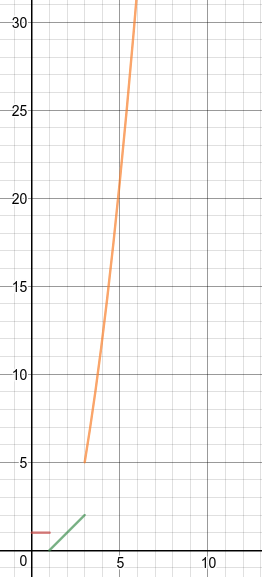
\includegraphics[width=6cm]{assets/hw_09_23.png}
\end{center}

\subsubsection*{Exercise 28}
Determine whether \( f(t) \) is continuous, piecewise continuous, or neither
on \( [0,10] \) and sketch the graph of \( f(t) \).
\[ f(t) = \begin{cases}
  \frac{\sin(t)}{t}, \quad t\ne0 \\
  1, \quad t = 0
\end{cases} \]
\( f(t) \) is continuous and piecewise continuous.
\begin{center}
  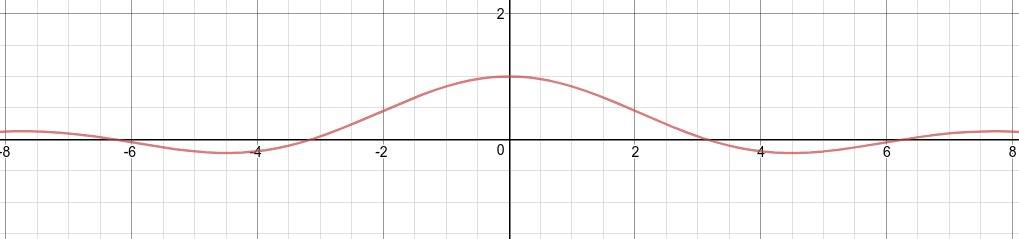
\includegraphics[width=16cm]{assets/hw_09_28.png}
\end{center}

\subsubsection*{Exercise 30}
For the transforms \( F(s) \) in Table 7.1, what can be said about
\( \lim_{s\to\infty}F(s) \)?
\par \( s \) is mostly in the denominator and increases in such a way that as
\( s\to\infty \), \( F(s) \) goes to 0.

\begin{center}
  If you have any questions, comments, or concerns, please contact me at
  alvin@omgimanerd.tech
\end{center}

\end{document}
